\section{Simulador}
\ \\ Al inciar la aplicacion se mostrará la siguiente pantalla:

\begin{figure}[htbp]
\begin{center}
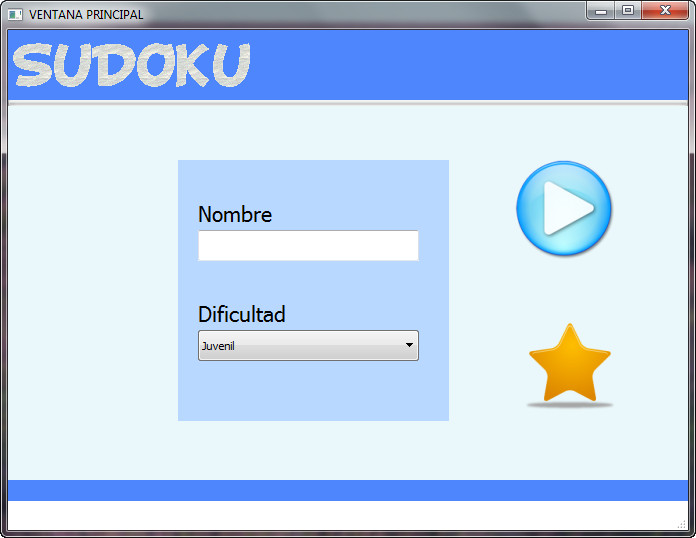
\includegraphics[width=.70\textwidth]{./imagenes/Inicio1.png}
\caption{Inicio}
\label{Inicio}
\end{center}
\end{figure}

\ \\ En donde deberá digitar el nombre de usuario con el que desee registrar su partida, y escoger uno de los 3 niveles de dificultad. \\ <Nota: Si no se escoge ningún nivel, por defecto se registrará el nivel Juvenil.>

\begin{figure}[htbp]
\begin{center}
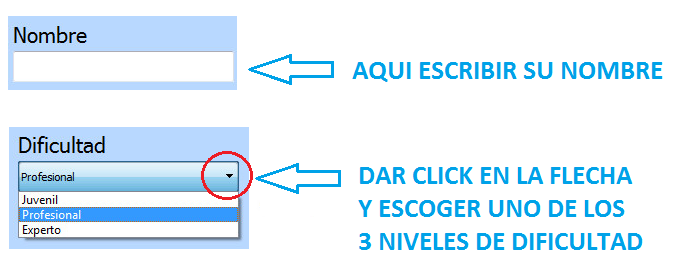
\includegraphics[width=.60\textwidth]{./imagenes/Inicio4.png}
\caption{Usuario y Nivel}
\label{Usuario y Nivel}
\end{center}
\end{figure}

\ \\ \ \\ 
Luego tenemos dos opciones: \\ 1. Presionar en \textbf{SCORE} para visualizar el ranking de las mejores puntuaciones, ó \\ 2. Presionar en \textbf{PLAY} para JUGAR. 

\begin{figure}[htbp]
\begin{center}
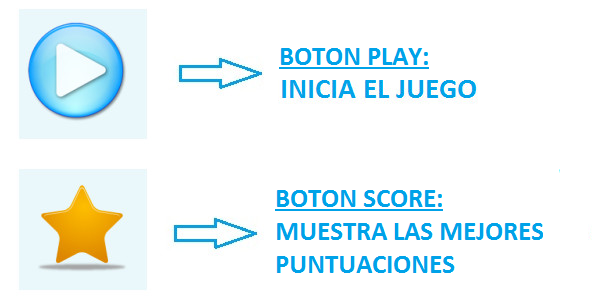
\includegraphics[width=.60\textwidth]{./imagenes/Controles.png}
\caption{Controles}
\label{Controles}
\end{center}
\end{figure} 

\ \\ \ \\
\textbf{Nota:} Para poder ver los \textbf{SCORE} no es necesario escribir un nombre de usuario, mientras que para poder \textbf{JUGAR} si es obligatorio escribir un nombre de usuario que además sea valido, caso contrario le apareceran los siguientes mensajes de error:

\begin{figure}[htbp]
\begin{center}
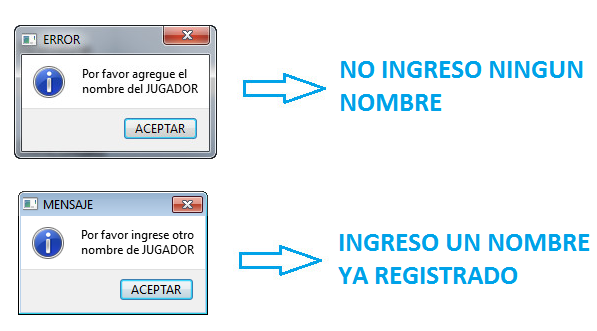
\includegraphics[width=.60\textwidth]{./imagenes/ErrorNoJugador.png}
\caption{Errores de Usuario}
\label{Errores de Usuario}
\end{center}
\end{figure} 

\ \\ \ \\ \ \\ \ \\
Si estamos en la pantalla inicial (Figura 4.2), y si presionamos en \textbf{SCORE}, se mostrará la siguiente pantalla, en donde se podrá visualizar el ranking de los usuarios que pudieron resolver el juego en menor tiempo. 
 
\begin{figure}[htbp]
\begin{center}
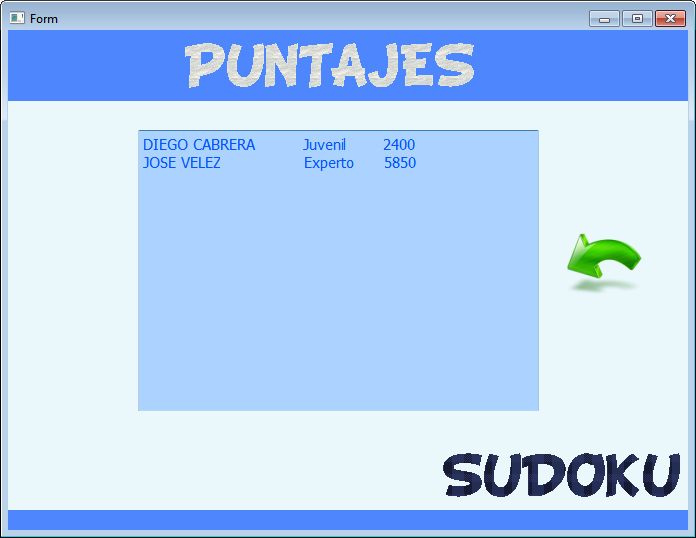
\includegraphics[width=.40\textwidth]{./imagenes/Puntajes3.png}
\caption{Puntuaciones}
\label{Puntuaciones}
\end{center}
\end{figure} 

\ \\ Para regresar al menu anterior (Figura 4.2) presionamos en \textbf{REGRESAR}.

\begin{figure}[htbp]
\begin{center}

\includegraphics[width=.40\textwidth]{./imagenes/Regresar.png}
\caption{Salir de Score}
\label{Salir de Score}
\end{center}
\end{figure} 

\ \\Sin embargo, si no hay puntajes guardados, la aplicación mostrará el siguiente mensaje de error:

\begin{figure}[htbp]
\begin{center}
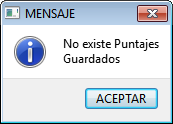
\includegraphics[width=.20\textwidth]{./imagenes/Puntajes2.png}
\caption{No hay Puntajes}
\label{No hay Puntajes}
\end{center}
\end{figure} 

\ \\Se deberá presionar en ACEPTAR para continuar.


\ \\ En el menú principal (Figura 4.2) si ahora presionamos en  \textbf{PLAY} entonces el juego iniciará y mostrará la siguiente pantalla:

\begin{figure}[htbp]
\begin{center}
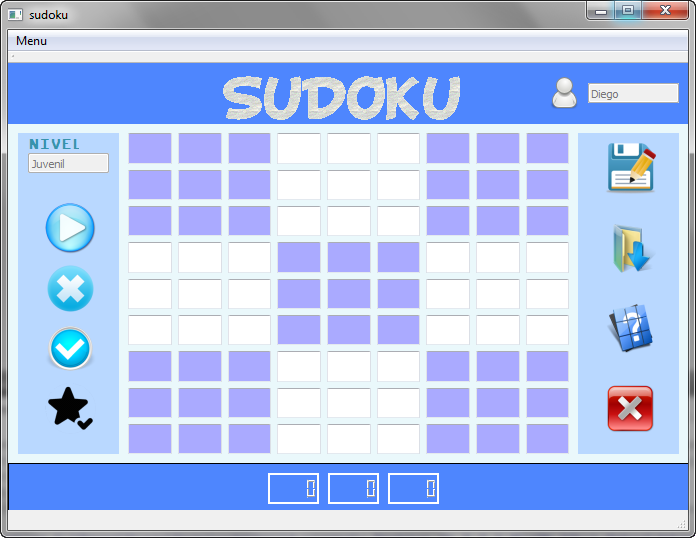
\includegraphics[width=.35\textwidth]{./imagenes/Sudoku.png}
\caption{Sudoku}
\label{Sudoku}
\end{center}
\end{figure} 

\ \\ Aqui tenemos varias opciones para poder jugar una partida de Sudoku, hay 3 paneles visuales en donde se muestra el usuario registrado, el nivel de dificultad y un cronometro que registra el tiempo transcurrido desde que se inicio la partida por el usuario.

\begin{figure}[htbp]
\begin{center}
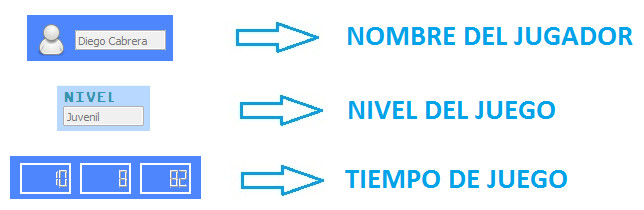
\includegraphics[width=.35\textwidth]{./imagenes/Panel.png}
\caption{Paneles de Información}
\label{Paneles de Información}
\end{center}
\end{figure} 

\ \\ Entre los controles principales del juego tenemos las opciones de: 

\begin{figure}[htbp]
\begin{center}
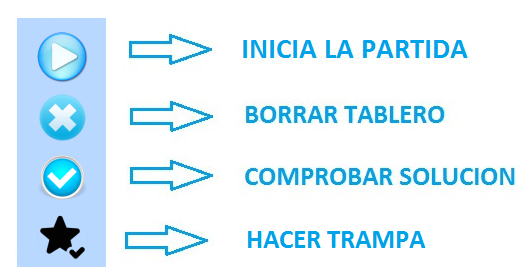
\includegraphics[width=.40\textwidth]{./imagenes/Controles1.png}
\caption{Controles Principales}
\label{Controles Principales}
\end{center}
\end{figure} 

\ \\ \ \\ \textbf{Iniciar la Partida:} Generá aleatoriamente el tablero del Sudoku con números ya dispuestos en algunas casillas y las demás casillas vacias, las cuales deben ser resueltas por el usuario \\ <Nota: Al inciar la partida, el CRONOMETRO empieza a contar.>  

\begin{figure}[htbp]
\begin{center}
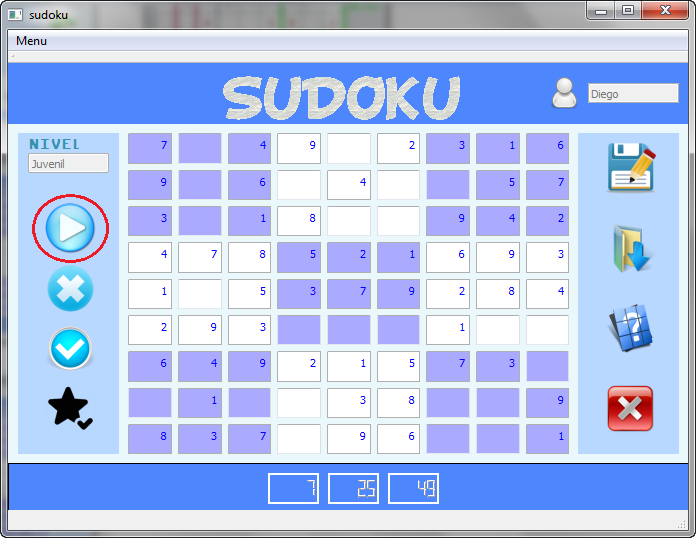
\includegraphics[width=.50\textwidth]{./imagenes/Tablero.png}
\caption{Tablero Aleatorio}
\label{Tablero}
\end{center}
\end{figure} 

\ \\ \textbf{Borrar el Tablero:} Nos ayuda a borrar toda los números del tablero.

\begin{figure}[htbp]
\begin{center}
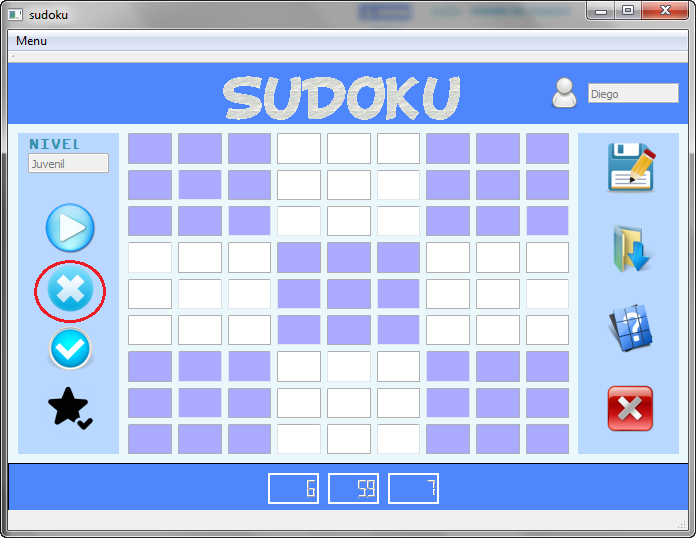
\includegraphics[width=.50\textwidth]{./imagenes/Tablero1.png}
\caption{Tablero Borrado}
\label{Tablero Borrado}
\end{center}
\end{figure} 

\ \\ \ \\ \ \\ \ \\
\textbf{Comprobar la Solución:} Luego de resolver el tablero, tenemos que presionar esta opción para que la aplicación nos indique si el tablero fue resuelto correctamente o no, de la siguiente manera:

\begin{figure}[htbp]
\begin{center}
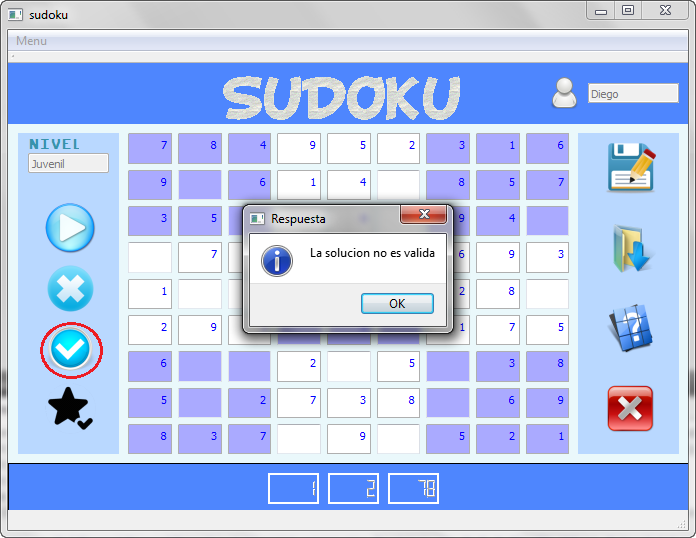
\includegraphics[width=.50\textwidth]{./imagenes/SudokuNo.png}
\caption{Sudoku Incorrecto}
\label{Sudoku Incorrecto}
\end{center}
\end{figure} 

\begin{figure}[htbp]
\begin{center}
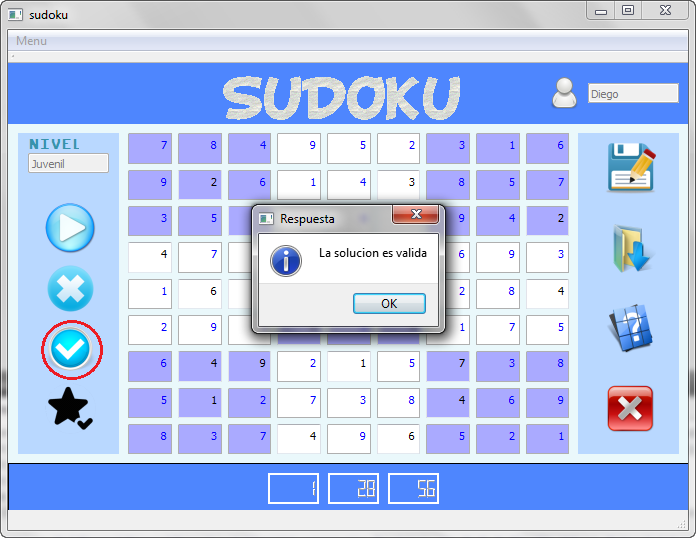
\includegraphics[width=.50\textwidth]{./imagenes/SudokuSi.png}
\caption{Sudoku Correcto}
\label{Sudoku Correcto}
\end{center}
\end{figure} 

\ \\ \ \\ \ \\ \ \\ \ \\ \ \\ \ \\
\textbf{Hacer Trampa:} Al escoger esta opción, el simulador mostrará alertas en las casillas en donde el valor digitado es correcto o incorrecto, de la siguiente manera: \\ <Verde: Correcto y Rosado: Incorrecto>


\begin{figure}[htbp]
\begin{center}
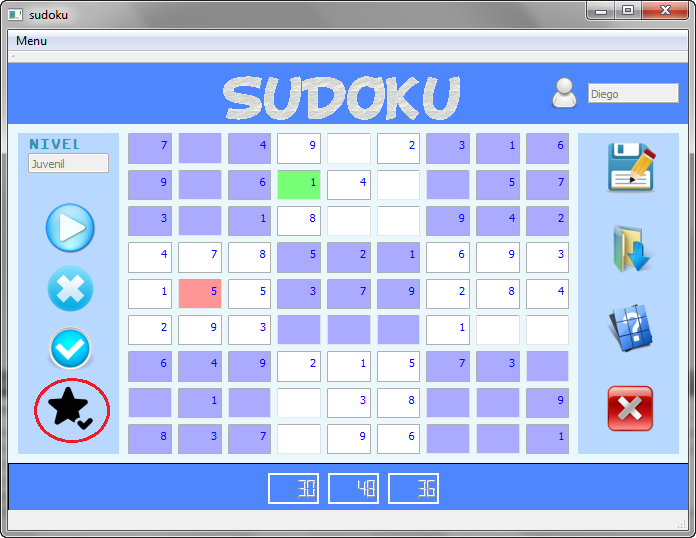
\includegraphics[width=.50\textwidth]{./imagenes/HacerTrampa.png}
\caption{Alertas}
\label{Alertas}
\end{center}
\end{figure} 

\ \\ También el simulador muestra ayudas automáticas para el usuario, en caso de que se digite un número que ya se encuentre en la fila o columna, mostrará el siguiente mensaje:

\begin{figure}[htbp]
\begin{center}
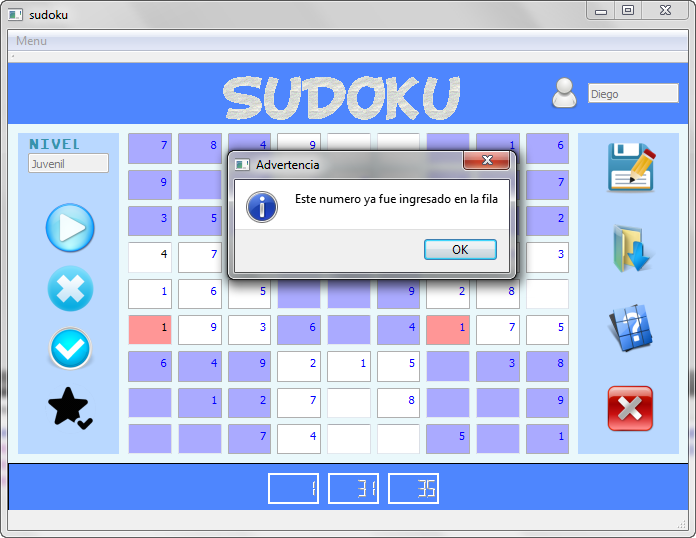
\includegraphics[width=.50\textwidth]{./imagenes/Pistas1.png}
\caption{Ayudas}
\label{Ayudas}
\end{center}
\end{figure} 

\ \\ \ \\ \ \\ \ \\ \ \\
Entre los demás controles del juego tenemos 4 opciones:

\begin{figure}[htbp]
\begin{center}
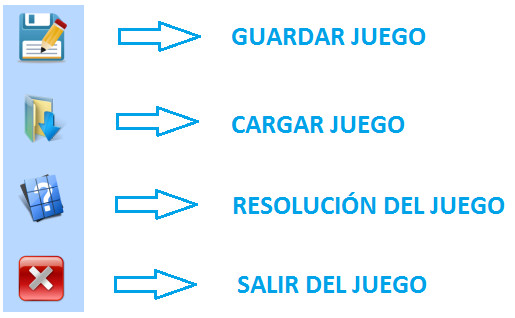
\includegraphics[width=.60\textwidth]{./imagenes/Controles2.png}
\caption{Controles Extras}
\label{Controles Extras}
\end{center}
\end{figure} 

\ \\ \textbf{1. Guardar Juego:} Guarda la partida del Sudoku, con todos los casilleros que se tienen resuelto hasta ese momento y el tiempo transcurrido. Al presionar esta opción, aparecerá el siguiente mensaje, donde se confirma que el juego se guardo correctamente. \\
<Nota: La partida se guardará con el nombe de usuario registrado al incio del juego.>
  
\begin{figure}[htbp]
\begin{center}
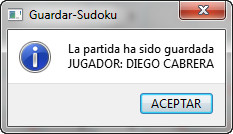
\includegraphics[width=.40\textwidth]{./imagenes/Guardar.png}
\caption{Juego Guardado}
\label{Juego Guardado}
\end{center}
\end{figure} 

\ \\ \ \\ \ \ \\ \ \\ 
\textbf{2. Cargar Juego:} Carga la partida del Sudoku con la misma información que tenía en el instante en el que fue guardada, es decir casilleros resueltos y tiempo transcurrido. Al presionar este botón, aparecerá la siguiente pantalla: \\ 
<Nota: Si algún usuario no ha guardado una partida con anterioridad, esta opción estará deshabilitada para dicho usuario.>

\begin{figure}[htbp]
\begin{center}
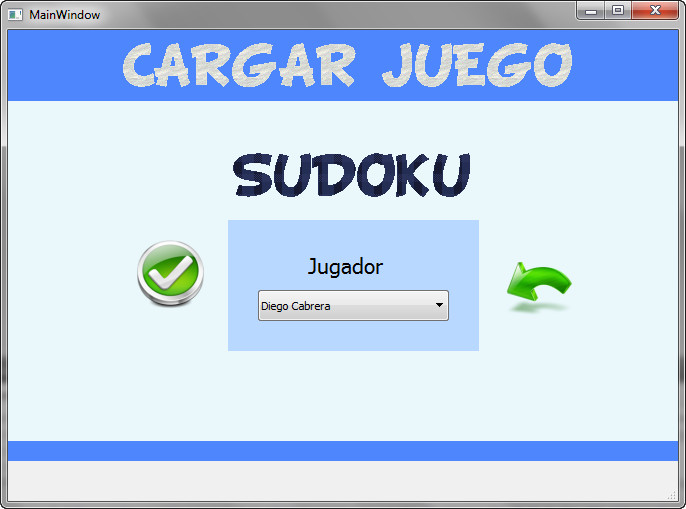
\includegraphics[width=.50\textwidth]{./imagenes/MenuCargar.png}
\caption{Cargar Juego}
\label{Cargar Juego}
\end{center}
\end{figure} 

\ \\ En la pantalla de \textbf{Cargar Juego} podemos visualizar la partida que esta guardada y debemos presionar el boton \textbf{CARGAR}, ó en caso de que el usuario ya no quisiera cargar su partida, se debe presionar el botón \textbf{REGRESAR} para volver al menú anterior.

\begin{figure}[htbp]
\begin{center}
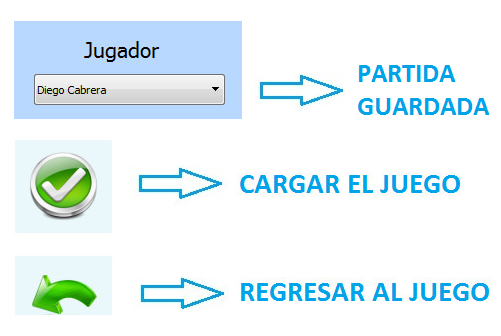
\includegraphics[width=.50\textwidth]{./imagenes/Controles3.png}
\caption{Controles Cargar Juego}
\label{Controles Cargar Juego}
\end{center}
\end{figure} 

\ \\ \ \\ \textbf{3. Solución del Juego:} Con esta opción, el Sudoku se resolverá por completo de forma automática. \\ <Nota: Al escoger esta opción, la partida será finalizada y no se contabilizará en el ranking de puntuaciones>

\begin{figure}[htbp]
\begin{center}
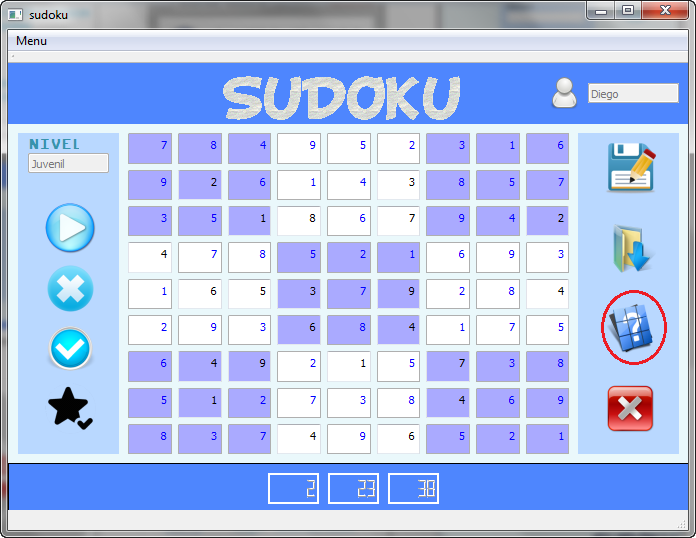
\includegraphics[width=.50\textwidth]{./imagenes/JuegoResuelto.png}
\caption{Juego Resuelto}
\label{Juego Resuelto}
\end{center}
\end{figure} 

\ \\ \textbf{4. Salir del Juego:} Con este botón podemos cerrar la aplicación, o también podemos utilizar la opción de la barra de Menú para poder salir del Juego.

\begin{figure}[htbp]
\begin{center}
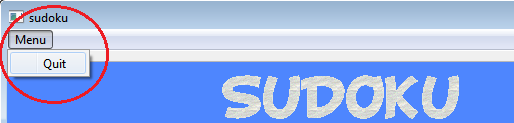
\includegraphics[width=.50\textwidth]{./imagenes/SeleccionMenu.png}
\caption{Menu Salir}
\label{Menu Salir}
\end{center}
\end{figure} 



